\section{Implementação, profiling e auditoria}\label{sec:impl}

Tudo foi implementado em Python~3.11 com NumPy. O NetworkX~\cite{hagberg2008}
é usado apenas no emparelhamento perfeito de peso mínimo do Christofides, e o
scikit-learn~\cite{pedregosa2011} apenas na análise. O código está organizado
em \texttt{tsp/}: leitor da TSPLIB, MST, heurísticas, aproximativos, B\&B,
features e profiler. Os experimentos ficam em \texttt{run\_*.py},
\texttt{profile\_scaling.py} e \texttt{audit\_naive.py}, e a análise em
\texttt{analise/}. Há 103 testes automatizados, que comparam com força
bruta, com o SciPy e com os ótimos e tours publicados da TSPLIB.

\subsection{Instâncias e distâncias}
O enunciado pede instâncias EUC\_2D com $N\in[10,75]$, mas a TSPLIB só tem
três nessa faixa (eil51, berlin52 e st70). Vários exemplos do próprio
enunciado são de outros tipos: ulysses16 é GEO, gr24, fri26 e swiss42 são
EXPLICIT, e att48 é ATT. Usamos 15 instâncias de 14 a 70 vértices
(Tabela~\ref{tab:instancias}), cada uma com a distância oficial do seu
tipo~\cite{reinelt1991}. A validação é que o custo de cada \texttt{.opt.tour}
publicado coincide com o ótimo publicado.

A regra de 80\% das instâncias com $N\le 40$ também não pode ser cumprida
com a TSPLIB, que só tem nove instâncias simétricas com $N\le40$. Usamos
todas as nove (60\% do conjunto). As instâncias EXPLICIT não têm
coordenadas. Para elas, coordenadas 2D foram obtidas por escalonamento
multidimensional clássico (MDS) da matriz de distâncias, e são usadas
\emph{apenas} nas features geométricas e na heurística do fecho convexo.
Para compensar o conjunto pequeno na análise de sensibilidade, geramos
instâncias sintéticas adversariais (Seção~\ref{sec:sens}).

\begin{table}[htb]
\centering
\caption{Instâncias da TSPLIB usadas. Geometria: origem das coordenadas das features geométricas. Viol. triangular: fração das triplas $(i,j,k)$ com $d(i,k)>d(i,j)+d(j,k)$.}
\label{tab:instancias}
\small
\begin{adjustbox}{max width=\linewidth}
\begin{tabular}{lrlrlrrr}
\toprule
Instância & $N$ & Tipo & Ótimo & Geometria & Fração no fecho & Clark-Evans & Viol. triangular \\
\midrule
burma14 & 14 & GEO & 3323 & coordenadas & 0{,}36 & 1{,}13 & 0{,}00\% \\
ulysses16 & 16 & GEO & 6859 & coordenadas & 0{,}44 & 1{,}10 & 0{,}00\% \\
gr17 & 17 & EXPLICIT & 2085 & MDS & 0{,}35 & 0{,}99 & 3{,}28\% \\
gr21 & 21 & EXPLICIT & 2707 & MDS & 0{,}38 & 1{,}10 & 2{,}61\% \\
ulysses22 & 22 & GEO & 7013 & coordenadas & 0{,}32 & 0{,}95 & 0{,}00\% \\
gr24 & 24 & EXPLICIT & 1272 & MDS & 0{,}29 & 1{,}18 & 4{,}61\% \\
fri26 & 26 & EXPLICIT & 937 & MDS & 0{,}35 & 1{,}09 & 0{,}17\% \\
bayg29 & 29 & EXPLICIT & 1610 & DISPLAY\_DATA & 0{,}24 & 1{,}33 & 0{,}00\% \\
bays29 & 29 & EXPLICIT & 2020 & DISPLAY\_DATA & 0{,}24 & 1{,}33 & 2{,}24\% \\
dantzig42 & 42 & EXPLICIT & 699 & DISPLAY\_DATA & 0{,}19 & 1{,}07 & 3{,}66\% \\
swiss42 & 42 & EXPLICIT & 1273 & MDS & 0{,}21 & 1{,}06 & 0{,}16\% \\
att48 & 48 & ATT & 10628 & coordenadas & 0{,}23 & 1{,}01 & 0{,}00\% \\
eil51 & 51 & EUC\_2D & 426 & coordenadas & 0{,}16 & 1{,}52 & 0{,}21\% \\
berlin52 & 52 & EUC\_2D & 7542 & coordenadas & 0{,}15 & 0{,}98 & 0{,}12\% \\
st70 & 70 & EUC\_2D & 675 & coordenadas & 0{,}14 & 1{,}04 & 0{,}23\% \\
\bottomrule
\end{tabular}
\end{adjustbox}
\end{table}


\subsection{Estruturas de dados e algoritmos}

\paragraph{Matriz de distâncias.} A matriz é densa ($n\times n$,
\texttt{float64}) e representa exatamente as distâncias inteiras da TSPLIB
(até $2^{53}$). Ela é \texttt{float} porque o limite de Held-Karp soma
penalidades reais. Uma cópia com $+\infty$ na diagonal evita testes
$i\neq j$ nos laços.

\paragraph{MST (Prim $O(n^2)$).} O grafo é completo, então Prim com vetor de
chaves é ótimo para grafo denso: $O(n^2)$, sem materializar as $n(n-1)/2$
arestas, como faria o Kruskal, e sem o $\log n$ do heap. Cada uma das $n$
iterações é uma operação vetorizada sobre o vetor de chaves.

\paragraph{Twice-around-the-tree.} Pré-ordem iterativa da MST (pilha
explícita), que equivale a percorrer cada aresta da árvore duas vezes e pular
os repetidos. O custo é $\le 2\,\mathrm{MST}\le 2\,\mathrm{OPT}$ sob a
desigualdade triangular.

\paragraph{Christofides~\cite{christofides1976}.} O algoritmo calcula a MST,
toma os vértices de grau ímpar ($k$ deles) e encontra um emparelhamento
perfeito de peso mínimo entre eles. Depois monta um circuito euleriano pelo
algoritmo de Hierholzer, com ponteiro por vértice para a próxima aresta
(cada aresta é examinada $O(1)$ vezes), e por fim aplica os atalhos. O
NetworkX só oferece emparelhamento de peso \emph{máximo} (blossom de
Edmonds~\cite{edmonds1965,galil1986}, $O(k^3)$). Usamos então
$w'(u,v)=C-d(u,v)$ com $C>\max d$ e \texttt{maxcardinality=True}: como todo
emparelhamento perfeito tem $k/2$ arestas, maximizar $\sum w'$ equivale a
minimizar $\sum d$. Também implementamos um emparelhamento guloso, que
escolhe as arestas em ordem crescente de peso em $O(k^2\log k)$, mas perde a
garantia de 1,5. Ele serve para medir o custo e a qualidade do blossom.

\paragraph{Heurísticas de warm-start.} São três:
\begin{itemize}
  \item \emph{trivial}: o tour $1\to2\to\dots\to n\to 1$;
  \item \emph{vizinho mais próximo}: $O(n^2)$, com máscara vetorizada dos
    visitados;
  \item \emph{inserção a partir do fecho convexo}: o fecho é calculado pela
    cadeia monótona de Andrew~\cite{andrew1979}, em $O(n\log n)$. Os
    vértices internos entram por inserção mais barata~\cite{rosenkrantz1977}.
    O tour é uma lista ligada (\texttt{succ}), e cada vértice de fora guarda
    em cache sua melhor inserção. Inserir $k$ entre $a$ e $b$ destrói só a
    aresta $(a,b)$, então só quem tinha $(a,b)$ como melhor aresta é
    recalculado contra o tour inteiro; os demais comparam apenas com as duas
    arestas novas.
\end{itemize}
Os aproximativos (TATT e Christofides) completam as cinco estratégias.

\subsection{Branch-and-Bound}

\paragraph{Espaço de busca.} Um nó é um caminho parcial
$P=(0,v_1,\dots,v_k)$, com $R$ o conjunto dos vértices não visitados. Fixar o
vértice inicial elimina as $n$ rotações equivalentes de cada tour. Os filhos
são $P+(c)$ para $c\in R$, e o nó com $|R|=1$ fecha o tour. Como os custos
são inteiros, um nó só melhora a incumbente $\mathrm{UB}$ se
$\lceil \mathrm{LB}\rceil\le \mathrm{UB}-1$; podamos quando
$\lceil\mathrm{LB}-10^{-6}\rceil\ge\mathrm{UB}$, com tolerância para o erro
de ponto flutuante.

\paragraph{Limites inferiores.} Todos são calculados para os $|R|$ filhos de
uma vez. Seja $R'=R\setminus\{c\}$.
\begin{itemize}
  \item \emph{Duas menores arestas} (\texttt{twomin}, o limite clássico
    de~\cite{levitin2012}). Somam-se, para cada vértice, as arestas fixadas
    no caminho ou as duas mais baratas incidentes a ele, e o total é dividido
    por 2.
  \item \emph{1-árvore} (\texttt{onetree}). Ainda falta um caminho
    hamiltoniano $c\to r_1\to\dots\to r_j\to 0$ passando por todo $R'$.
    Tirando as duas arestas das pontas, sobra uma árvore geradora de $R'$:
    \[
      \mathrm{LB}(c)=d(P)+d(v_k,c)+\mathrm{MST}(R')
      +\min_{r\in R'} d(c,r)+\min_{r\in R'} d(r,0).
    \]
  \item \emph{Held-Karp} (\texttt{hk})~\cite{heldkarp1970,heldkarp1971}. É o
    mesmo limite sobre os custos penalizados $w_{ij}=d_{ij}+\pi_i+\pi_j$.
    Todo tour tem grau 2 em todo vértice, então
    $w(\text{tour})=d(\text{tour})+2\sum\pi$, e qualquer limite em $w$ vale
    para $d$ subtraindo $2\sum\pi$. As penalidades são otimizadas uma única
    vez, na raiz, por subgradiente da relaxação Lagrangiana da 1-árvore:
    $g_v=\mathrm{grau}_v-2$ e passo de Polyak
    $t=\lambda(\mathrm{UB}-L(\pi))/\lVert g\rVert^2$. O $\lambda$ começa em 2
    e cai pela metade após $\max(5,n/5)$ iterações sem melhora, com no máximo
    $50n$ iterações. O UB que calibra o passo é sempre o do vizinho mais
    próximo, para que o limite (e portanto a poda) não dependa do warm-start.
\end{itemize}
Os limites dos filhos exigem $\mathrm{MST}(R\setminus\{c\})$ para cada
$c\in R$. Em vez de $|R|$ execuções do Prim, com $|R|^2$ iterações do
interpretador, rodamos os $|R|$ Prims \emph{em lote}. Uma matriz de chaves
$|R|\times|R|$ é relaxada com uma operação NumPy por iteração, de modo que o
laço Python tem $|R|-2$ iterações. O custo aritmético continua
$O(|R|^3)$ por nó.

\paragraph{Estratégia de busca.} A estratégia padrão é a busca em
profundidade (DFS) recursiva, com um único vetor booleano de visitados e um
único caminho, ambos modificados no lugar. A memória é $O(n^2)$ (pilha de
recursão mais um vetor de limites por nível), contra a memória exponencial
do best-first. Os filhos podem ser visitados em ordem crescente de LB
(\emph{filhos por LB}), o que dá à DFS um comportamento parecido com o do
best-first, ou na ordem dos índices (\emph{filhos por índice}). No segundo
caso, a DFS depende só do UB para podar, o que isola o efeito do warm-start.
Com filhos ordenados, ao podar um filho podamos também todos os irmãos
seguintes. O best-first também está implementado: um heap ordenado por
$(\mathrm{LB},-\text{profundidade})$, com o caminho guardado como lista
encadeada imutável e um teto de 2 milhões de nós abertos. Ele aparece só na
auditoria. Em todas as estratégias valem os invariantes
gerados $=$ podados $+$ expandidos $+$ folhas, conferidos nos testes.

\subsection{Instrumentação}
\begin{itemize}
  \item \emph{Seções.} Cada subrotina roda dentro de
    \texttt{prof.section(nome)}. São elas: MST, pré-ordem, vértices ímpares,
    construção do grafo do matching, blossom, Hierholzer, atalhos, fecho e
    inserção; no B\&B, o limite na raiz e os limites dos filhos.
  \item \emph{Tempo.} É medido com \texttt{perf\_counter}: uma execução de
    aquecimento descartada seguida da mediana de 5 repetições (3 nas
    instâncias aleatórias).
  \item \emph{Memória.} O \texttt{tracemalloc} deixa o Python várias vezes
    mais lento, então a memória é medida numa execução \emph{separada}. Cada
    seção registra o pico de alocação acima do que já estava alocado ao
    entrar nela, após um \texttt{gc.collect()}.
  \item \emph{Memória do B\&B.} O RSS do processo não serve: os
    $\approx$170~MiB do interpretador e das bibliotecas escondem os KiB da
    DFS (o RSS extra deu zero nas 300 execuções). Usamos por isso uma
    execução curta sob \texttt{tracemalloc}. A DFS atinge o pico logo no
    primeiro mergulho.
  \item \emph{Isolamento.} Cada execução de B\&B roda num subprocesso. Além
    do tempo de relógio, registramos o tempo de CPU do processo, para
    quantificar a contenção quando há processos em paralelo. As bibliotecas
    numéricas usam 1 thread.
  \item \emph{GC.} As coletas do garbage collector são contadas apenas
    dentro da janela cronometrada. Todos os experimentos de tempo foram
    repetidos com o GC desligado.
\end{itemize}

\subsection{Auditoria e refatorações}\label{sec:auditoria}
O módulo \texttt{tsp/naive.py} reconstrói, como linha de base, os padrões de
código ingênuo que um LLM tipicamente entrega sem revisão. São eles:
\begin{itemize}
  \item best-first que copia o caminho inteiro em cada filho, testa
    pertinência com \texttt{v in path} em lista ($O(n)$) e recalcula o
    limite do zero em Python puro ($O(n^2)$ por nó);
  \item TATT e Christofides sobre o grafo \emph{completo} do NetworkX
    ($n(n-1)/2$ arestas como dicionários);
  \item circuito euleriano via \texttt{MultiGraph}.
\end{itemize}
O script \texttt{audit\_naive.py} mede as duas versões nas mesmas
condições (Tabelas~\ref{tab:auditoria_aprox} e~\ref{tab:auditoria_bnb},
Figura~\ref{fig:auditoria_mst}).

\paragraph{Aproximativos.} No TATT, trocar o grafo do NetworkX pelo Prim
$O(n^2)$ sobre a matriz deu 89$\times$ menos tempo e 714$\times$ menos
memória em $N=500$ (49~MiB contra 0,07~MiB). No Christofides o ganho de
tempo é pequeno (1,1 a 2,1$\times$), e foi o \emph{profiling por
subrotina} que mostrou por quê: o blossom domina as duas versões. Ele
responde por 81\% do tempo já em $N=25$ e por praticamente 100\% em
$N=1000$ (Figura~\ref{fig:tempo}b). A refatoração reduziu a memória em 3,8
a 7,2$\times$, porque o grafo do matching agora tem só os $k$ vértices
ímpares, e não mais os $n$ vértices. Mais tempo nas outras subrotinas não
mudaria o total: o próximo passo seria um matching em C, ou o guloso, que
custa 2$\times$ mais gap (Seção~\ref{sec:sens}).

\begin{figure}[htb]
\centering
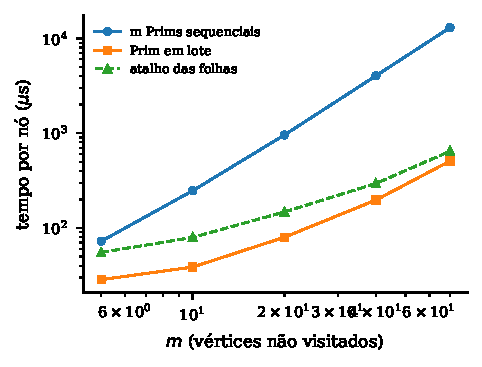
\includegraphics[width=0.5\textwidth]{auditoria_children_mst}
\caption{Tempo para calcular $\mathrm{MST}(R\setminus\{c\})$ para todos os
$m$ filhos de um nó: $m$ execuções sequenciais do Prim, Prim em lote e atalho
das folhas.}\label{fig:auditoria_mst}
\end{figure}

\paragraph{Limites dos filhos no B\&B.} O profiling do B\&B
(Tabela~\ref{tab:perfil}) mostrou que, nas configurações em que a árvore é
grande, 83 a 94\% do tempo vai para o cálculo dos limites dos filhos. Com
Held-Karp e filhos por LB, as árvores são tão pequenas que metade do tempo
vai para o subgradiente na raiz. O Prim em lote foi
25$\times$ mais rápido que $m$ execuções sequenciais em $m=70$ (0,51~ms
contra 12,96~ms). A revisão cruzada sugeriu ainda o \emph{atalho das
folhas}: se $c$ é folha da MST $T$ de $R$, então $T-c$ é MST de $R-c$, e
o limite sai em $O(1)$. A propriedade é verdadeira, e a implementação bate
com o Prim sequencial nos testes. Mesmo assim, ela foi 1,3 a 2,1$\times$
\emph{mais lenta} que o lote para $m\le70$. O atalho exige um Prim extra
com $m$ iterações do interpretador, e nesse tamanho o custo é dominado pelo
número de iterações Python, não pela aritmética, que o NumPy faz em
microssegundos. É um exemplo direto de gargalo teórico que não é o gargalo
prático, por isso a versão em lote continuou como padrão.

\begin{table}[htb]
\centering
\caption{Auditoria dos aproximativos: versão bruta (grafo completo no NetworkX) x refatorada (Prim $O(n^2)$ na matriz, matching só nos vértices ímpares). Tempo: mediana de 3 execuções; memória: pico do tracemalloc.}
\label{tab:auditoria_aprox}
\small
\begin{adjustbox}{max width=\linewidth}
\begin{tabular}{lrlrrrrr}
\toprule
Caso & $N$ & Algoritmo & Tempo bruto (ms) & Tempo ref. (ms) & Speedup & Mem. bruto (MiB) & Mem. ref. (MiB) \\
\midrule
gr24 & 24 & TATT & 0{,}39 & 0{,}08 & 5{,}0$\times$ & 0{,}13 & 0{,}01 \\
gr24 & 24 & Christofides & 1{,}37 & 0{,}66 & 2{,}1$\times$ & 0{,}21 & 0{,}05 \\
att48 & 48 & TATT & 1{,}30 & 0{,}14 & 9{,}0$\times$ & 0{,}46 & 0{,}01 \\
att48 & 48 & Christofides & 9{,}91 & 7{,}02 & 1{,}4$\times$ & 0{,}68 & 0{,}18 \\
st70 & 70 & TATT & 2{,}67 & 0{,}21 & 12{,}7$\times$ & 0{,}90 & 0{,}02 \\
st70 & 70 & Christofides & 11{,}39 & 8{,}08 & 1{,}4$\times$ & 1{,}11 & 0{,}23 \\
random200 & 200 & TATT & 22{,}74 & 0{,}64 & 35{,}5$\times$ & 7{,}78 & 0{,}03 \\
random200 & 200 & Christofides & 155{,}71 & 117{,}47 & 1{,}3$\times$ & 7{,}78 & 1{,}09 \\
random500 & 500 & TATT & 170{,}03 & 1{,}90 & 89{,}4$\times$ & 48{,}94 & 0{,}07 \\
random500 & 500 & Christofides & 2.551{,}72 & 2.221{,}46 & 1{,}1$\times$ & 48{,}94 & 8{,}86 \\
\bottomrule
\end{tabular}
\end{adjustbox}
\end{table}

\begin{table}[htb]
\centering
\caption{Auditoria do B\&B (limite de 30 s por execução; todas as variantes com o mesmo warm-start, vizinho mais próximo, e o mesmo teto de 2 milhões de nós abertos). B/nó aberto: pico de memória dividido pelo máximo de nós abertos, ambos da mesma execução com tracemalloc.}
\label{tab:auditoria_bnb}
\small
\begin{adjustbox}{max width=\linewidth}
\begin{tabular}{llcrrrr}
\toprule
Instância & Variante & Status & Nós exp. & Tempo (s) & Pico (MiB) & B/nó aberto \\
\midrule
burma14 & bruto: best-first, cópias, LB em Python & ótimo & 483.341 & 18{,}13 & 101{,}2 & 259 \\
burma14 & bruto, GC desligado & ótimo & 483.341 & 17{,}78 & 101{,}3 & 260 \\
burma14 & best-first refatorado & ótimo & 237.333 & 3{,}66 & 98{,}1 & 273 \\
burma14 & best-first refatorado, GC desligado & ótimo & 237.333 & 3{,}46 & 98{,}1 & 273 \\
burma14 & DFS, 2 menores arestas & ótimo & 278.533 & 3{,}35 & 0{,}0 & -- \\
burma14 & DFS, 1-árvore & ótimo & 7.772 & 0{,}24 & 0{,}0 & -- \\
burma14 & DFS, Held-Karp & ótimo & 12 & 0{,}00 & 0{,}0 & -- \\
ulysses16 & bruto: best-first, cópias, LB em Python & memória & 337.320 & 27{,}26 & 104{,}0 & 257 \\
ulysses16 & bruto, GC desligado & memória & 337.320 & 25{,}18 & 103{,}9 & 257 \\
ulysses16 & best-first refatorado & memória & 311.106 & 6{,}84 & 365{,}7 & 268 \\
ulysses16 & best-first refatorado, GC desligado & memória & 311.106 & 5{,}75 & 368{,}4 & 268 \\
ulysses16 & DFS, 2 menores arestas & timeout & 2.497.158 & 30{,}00 & 0{,}0 & -- \\
ulysses16 & DFS, 1-árvore & timeout & 1.092.828 & 30{,}00 & 0{,}0 & -- \\
ulysses16 & DFS, Held-Karp & ótimo & 14 & 0{,}01 & 0{,}0 & -- \\
gr17 & bruto: best-first, cópias, LB em Python & timeout & 327.115 & 30{,}42 & 94{,}9 & 260 \\
gr17 & bruto, GC desligado & timeout & 347.969 & 30{,}45 & 95{,}2 & 260 \\
gr17 & best-first refatorado & memória & 419.819 & 8{,}89 & 323{,}4 & 270 \\
gr17 & best-first refatorado, GC desligado & memória & 419.819 & 7{,}72 & 322{,}0 & 270 \\
gr17 & DFS, 2 menores arestas & timeout & 2.426.378 & 30{,}00 & 0{,}0 & -- \\
gr17 & DFS, 1-árvore & ótimo & 293.064 & 10{,}62 & 0{,}0 & -- \\
gr17 & DFS, Held-Karp & ótimo & 15 & 0{,}00 & 0{,}0 & -- \\
\bottomrule
\end{tabular}
\end{adjustbox}
\end{table}


\paragraph{Estratégia da árvore: best-first $\times$ DFS.} Com o mesmo
limite fraco (duas menores arestas), o mesmo warm-start e o mesmo teto de
nós abertos, o best-first refatorado resolveu o burma14 em 3,7~s, contra
18,1~s da versão bruta. Ele expandiu metade dos nós (237 mil contra 483
mil), porque o limite refatorado restringe as arestas livres das pontas do
caminho aos vértices não visitados. Nas duas versões, porém, cada nó aberto
custa cerca de 260 a 270~bytes, e a fila chega a centenas de MiB. No
ulysses16 e no gr17, o best-first estourou o teto de 2 milhões de nós
abertos (320 a 370~MiB) em menos de 10~s. A DFS com o mesmo limite usou
0,03~MiB nas três instâncias. Por isso a DFS é a estratégia padrão: a
memória cai de exponencial para $O(n^2)$, e a perda (expandir nós que o
best-first não expandiria) é compensada por um bom limite. Com Held-Karp, a
DFS resolveu as três instâncias expandindo 12 a 15 nós em menos de 10~ms.
Para o best-first, guardar o caminho como lista encadeada (filho em $O(1)$)
reduziu o custo por nó de $\approx$340 para $\approx$270~bytes. O restante
é o custo fixo de uma tupla Python com 6 campos.

